\documentclass[border=12pt]{standalone}
\usepackage{tikz}
\usetikzlibrary{shapes.geometric, arrows.meta, positioning, calc, fit, backgrounds}
\usepackage{fontspec}
\setmainfont{DejaVu Sans}

\begin{document}
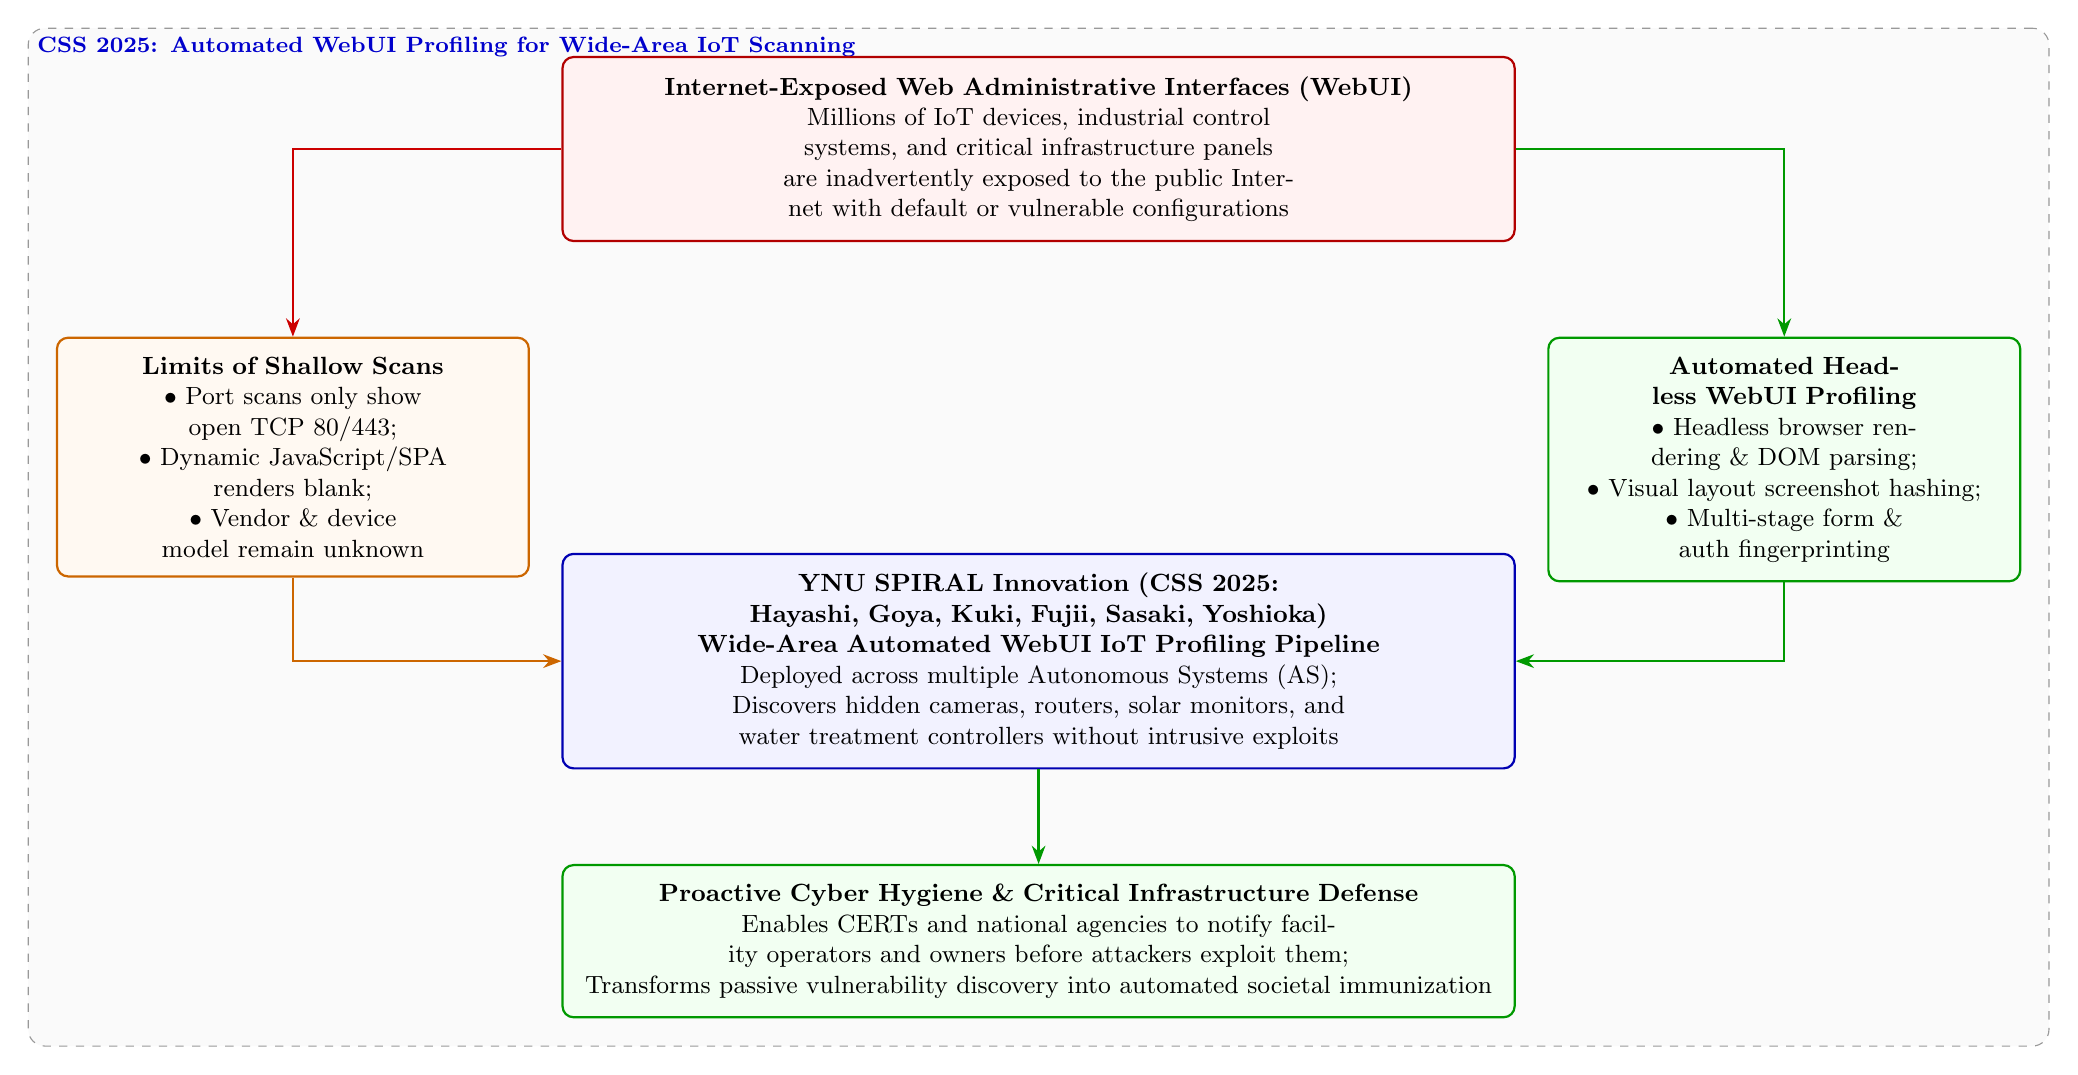
\begin{tikzpicture}[
    font=\small,
    >=Stealth,
    node distance=1.2cm,
    block/.style={rectangle, draw=blue!70!black, fill=blue!5, rounded corners=4pt, thick, align=center, inner sep=7pt},
    alertblock/.style={rectangle, draw=red!70!black, fill=red!5, rounded corners=4pt, thick, align=center, inner sep=7pt},
    greenblock/.style={rectangle, draw=green!60!black, fill=green!5, rounded corners=4pt, thick, align=center, inner sep=7pt},
    amberblock/.style={rectangle, draw=orange!80!black, fill=orange!5, rounded corners=4pt, thick, align=center, inner sep=7pt},
    groupbox/.style={draw=black!40, dashed, rounded corners=6pt, fill=black!2, inner sep=10pt}
]

    % Top: The Internet-Wide Exposure
    \node[alertblock, text width=11.6cm] (exposure) {\textbf{Internet-Exposed Web Administrative Interfaces (WebUI)}\\Millions of IoT devices, industrial control systems, and critical infrastructure panels\\are inadvertently exposed to the public Internet with default or vulnerable configurations};

    % Left: Challenge of Traditional Port Scanning
    \node[amberblock, below left=1.2cm and 0.4cm of exposure, text width=5.5cm] (challenge) {\textbf{Limits of Shallow Scans}\\$\bullet$ Port scans only show open TCP 80/443;\\$\bullet$ Dynamic JavaScript/SPA renders blank;\\$\bullet$ Vendor \& device model remain unknown};

    % Right: Autonomous Profiling Pipeline
    \node[greenblock, below right=1.2cm and 0.4cm of exposure, text width=5.5cm] (solution) {\textbf{Automated Headless WebUI Profiling}\\$\bullet$ Headless browser rendering \& DOM parsing;\\$\bullet$ Visual layout screenshot hashing;\\$\bullet$ Multi-stage form \& auth fingerprinting};

    \draw[->, thick, red!80!black] (exposure) -| (challenge);
    \draw[->, thick, green!60!black] (exposure) -| (solution);

    % Middle: YNU Research Breakthrough (CSS 2025)
    \node[block, below=1.2cm of $(challenge)!0.5!(solution)$, text width=11.6cm] (breakthrough) {\textbf{YNU SPIRAL Innovation (CSS 2025: Hayashi, Goya, Kuki, Fujii, Sasaki, Yoshioka)}\\\textbf{Wide-Area Automated WebUI IoT Profiling Pipeline}\\Deployed across multiple Autonomous Systems (AS);\\Discovers hidden cameras, routers, solar monitors, and water treatment controllers without intrusive exploits};

    \draw[->, thick, orange!80!black] (challenge) |- (breakthrough);
    \draw[->, thick, green!60!black] (solution) |- (breakthrough);

    % Bottom: National & Global Impact
    \node[greenblock, below=1.2cm of breakthrough, text width=11.6cm] (impact) {\textbf{Proactive Cyber Hygiene \& Critical Infrastructure Defense}\\Enables CERTs and national agencies to notify facility operators and owners before attackers exploit them;\\Transforms passive vulnerability discovery into automated societal immunization};

    \draw[->, thick, green!60!black] (breakthrough) -- (impact);

    \begin{scope}[on background layer]
        \node[groupbox, fit=(exposure) (challenge) (solution) (breakthrough) (impact), label={[anchor=north west, font=\footnotesize\bfseries, blue!80!black]north west:CSS 2025: Automated WebUI Profiling for Wide-Area IoT Scanning}] {};
    \end{scope}

\end{tikzpicture}
\end{document}
